\chapter{분포 (Distribution)}
\label{descriptive}


\section{히스토그램}
\label{histograms}

변수를 기술하는 가장 좋은 방법중의 하나는 데이터셋에 나타나는 값과
각 값이 얼마나 나타나는지를 보고하는 것이다.
이러한 기술법을 변수 {\bf 분포(distribution)}라고 부른다.
\index{분포 (distribution)}

가장 일반적인 분포 표현은 {\bf 히스토그램(histogram)}으로 각 값의 
{\bf 빈도(frequency)}를 보여주는 그래프다. 이러한 맥락에서 ``빈도''는
값이 출현하는 횟수를 의미한다. 
\index{히스토그램 (histogram)} 
\index{빈도 (frequency)}
\index{딕셔러리 (dictionary)}

파이썬에서 빈도를 계산하는 효율적인 방법은 딕셔너리를 사용하는 것이다.
시퀀스 값 {\tt t}가 주어진 상태에서,
%
\begin{verbatim}
hist = {}
for x in t:
    hist[x] = hist.get(x, 0) + 1
\end{verbatim}

결과는 값을 빈도로 매칭하는 딕셔너리다. 대안으로 
{\tt collections} 모듈에 정의된 {\tt Counter} 클래스를 사용할 수 있다.


\begin{verbatim}
from collections import Counter
counter = Counter(t)
\end{verbatim}

결과는 {\tt Counter} 객체로 딕셔너리의 하위클래스가 된다.

또다른 선택지는 판다스 \verb"value_counts" 메쏘드를 사용하는 것으로 앞장에서 살펴봤다.
하지만, 이 책에서 히스토그램을 나타내는 Hist 클래스를 생성하고 Hist 클래스에서 동작하는 메쏘드를 제공한다.

\index{판다스 (pandas)}


\section{히스토그램 표현하기}
\index{히스토그램 (histogram)}
\index{Hist}

Hist 생성자는 시퀀스, 딕셔너리, 판다스 시리즈, 혹은 다른 Hist를 받을 수 있다.
다음과 같이 Hist 객체 인스턴스를 생성할 수 있다.

%
\begin{verbatim}
>>> import thinkstats2
>>> hist = thinkstats2.Hist([1, 2, 2, 3, 5])
>>> hist
Hist({1: 1, 2: 2, 3: 1, 5: 1})
\end{verbatim}

Hist 객체는 {\tt Freq} 메쏘드를 제공하는데 값을 받아 빈도를 반환한다.
\index{빈도 (frequency)}

%
\begin{verbatim}
>>> hist.Freq(2)
2
\end{verbatim}

꺾쇠 연산자도 동일한 것을 수행한다.
\index{꺾쇠 연산자 (bracket operator)}

%
\begin{verbatim}
>>> hist[2]
2
\end{verbatim}

만약 찾는 값이 없다면, 빈도는 0이다.

%
\begin{verbatim}
>>> hist.Freq(4)
0
\end{verbatim}

{\tt Values} 메쏘드는 Hist에 정렬되지 않는 리스트 값을 반환한다.
%
\begin{verbatim}
>>> hist.Values()
[1, 5, 3, 2]
\end{verbatim}

정렬된 값으로 루프를 돌리려면, 내장함수 {\tt sorted}를 사용할 수 있다.

%
\begin{verbatim}
for val in sorted(hist.Values()):
    print(val, hist.Freq(val))
\end{verbatim}

{\tt Items} 메쏘드를 사용해서 값-빈도(value-frequency) 짝을 반복처리할 수 있다.

%
\begin{verbatim}
for val, freq in hist.Items():
     print(val, freq)
\end{verbatim}


\section{히스토그램 그리기 (Plotting histograms)}
\index{pyplot}

\begin{figure}
% first.py
\centerline{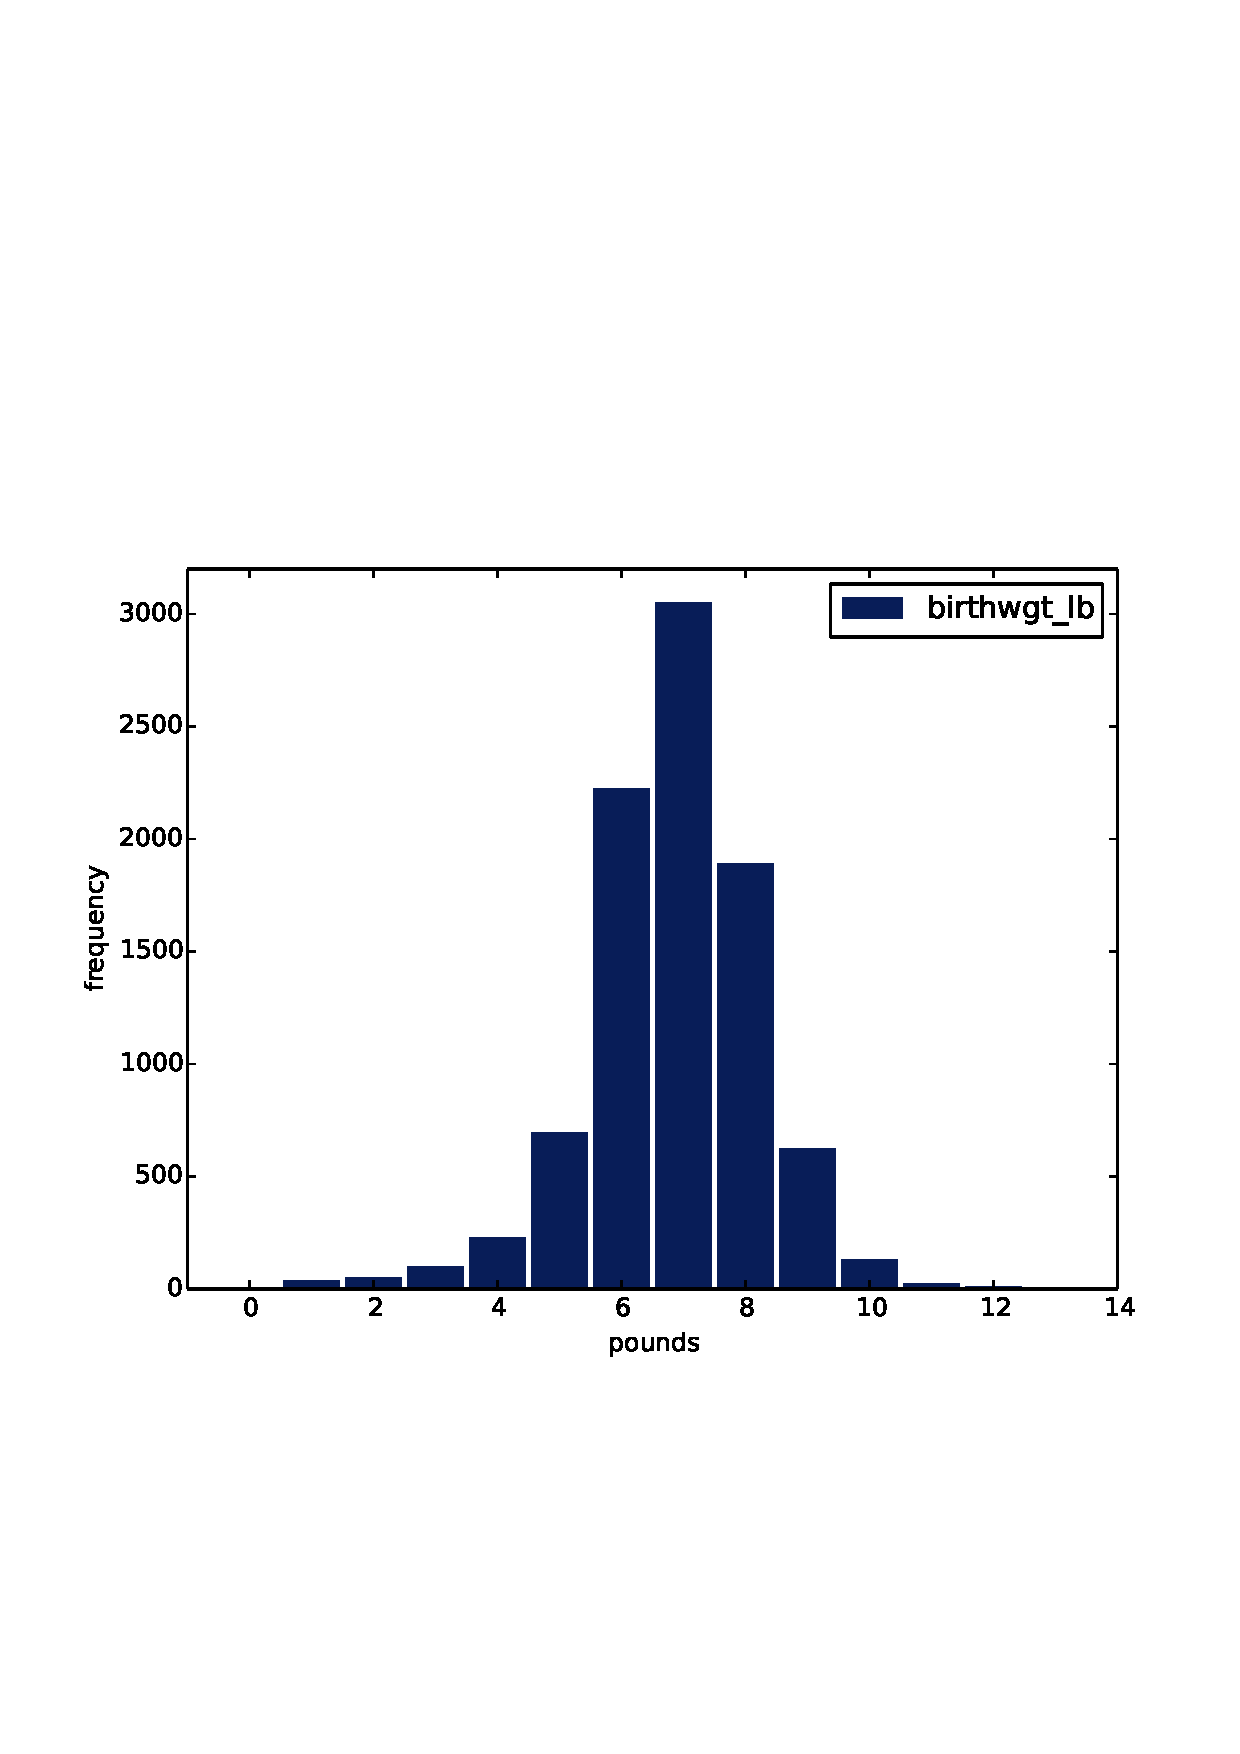
\includegraphics[height=2.5in]{figs/first_wgt_lb_hist.pdf}}
\caption{출생체중 파운드 히스토그램.}
\label{first_wgt_lb_hist}
\end{figure}

이 책에서 저자는 {\tt thinkplot.py} 모듈을 작성해서 Hists를 그리는 함수와 
{\tt thinkstats2.py}에 정의된 객체를 제공한다. {\tt pyplot}에 기반하고 있고 
{\tt matplotlib} 패키지의 일부다. 
{\tt matplotlib}을 설치하는 방법은 ~\ref{code}을 참조하세요.

\index{thinkplot}
\index{matplotlib}

{\tt thinkplot}으로 {\tt hist}를 그리기 위해서 다음을 시도해 보세요.

\index{Hist}

\begin{verbatim}
>>> import thinkplot
>>> thinkplot.Hist(hist)
>>> thinkplot.Show(xlabel='value', ylabel='frequency')
\end{verbatim}

\url{http://greenteapress.com/thinkstats2/thinkplot.html} 웹사이트에서
{\tt thinkplot}에 대한 문서를 참조할 수 있다.

\begin{figure}
% first.py
\centerline{\includegraphics[height=2.5in]{figs/first_wgt_oz_hist.pdf}}
\caption{출생체중 온스 히스토그램.}
\label{first_wgt_oz_hist}
\end{figure}


\section{NSFG 변수}

이제 NSFG에 있는 데이터로 다시 돌아가자. 이장에 있는 코드는 {\tt first.py}다. 
코드를 다운로드하고 작업에 대한 정보는 ~\ref{code} 장을 참조하라.

새로운 데이터셋을 가지고 작업을 시작할 때, 한번에 하나씩 사용하려는 변수를 탐색하길 제안한다. 
시작하는 좋은 방법은 히스토그램을 그려보는 것이다.

\index{히스토그램 (histogram)}


~\ref{cleaning}에서 {\tt agepreg}를 백분년에서 년단위로 변환했고,
\verb"birthwgt_lb"와 \verb"birthwgt_oz"을 조합해서 \verb"totalwgt_lb" 한 단위량으로 만들었다.
이번 절에서 히스토그램의 몇가지 기능을 시연하기 위해서 이 변수들을 사용한다.


\begin{figure}
% first.py
\centerline{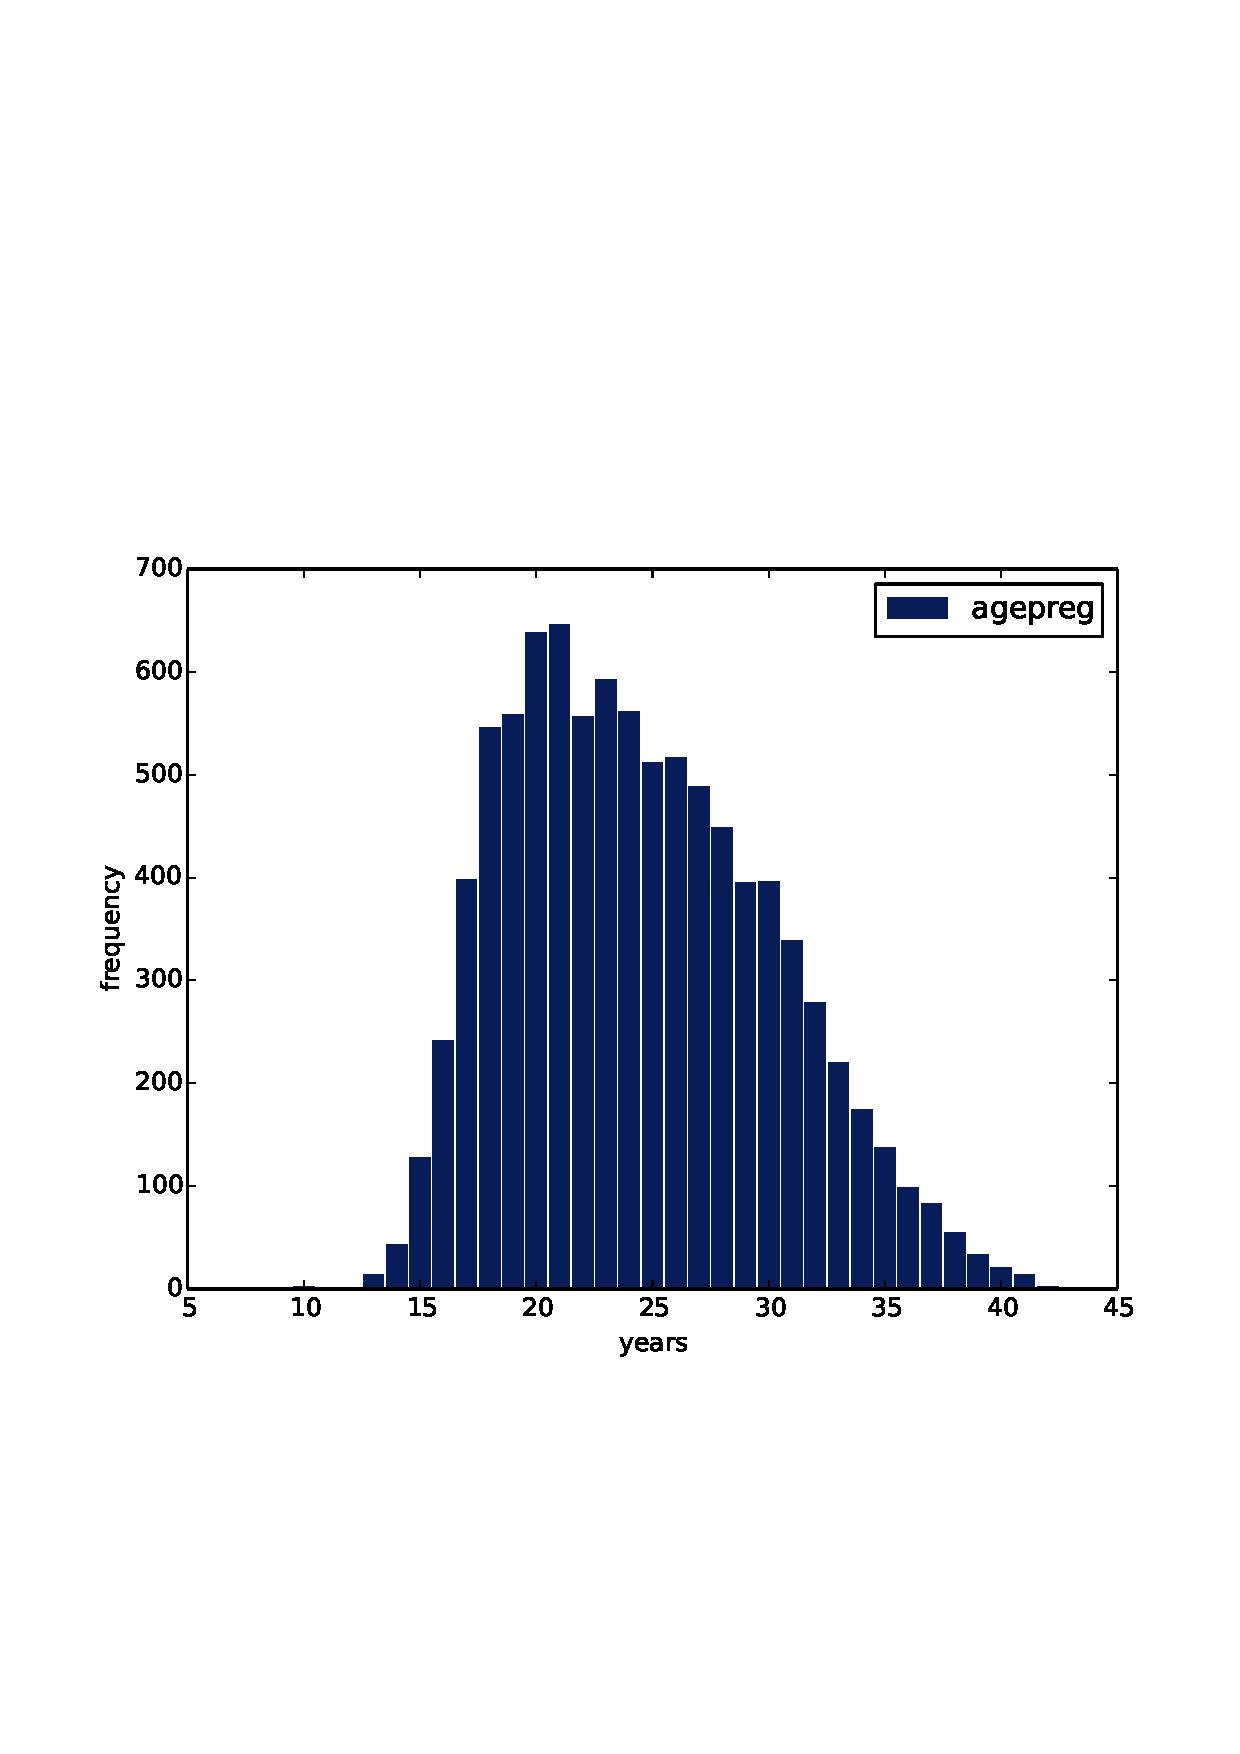
\includegraphics[height=2.5in]{figs/first_agepreg_hist.pdf}}
\caption{임신 종료시점 산모연령 히스토그램.}
\label{first_agepreg_hist}
\end{figure}

데이터를 읽고, 정상 출산에 대한 레코드를 선택해서 시작해보자.

\begin{verbatim}
    preg = nsfg.ReadFemPreg()
    live = preg[preg.outcome == 1]
\end{verbatim}

꺾쇠 표현식은 부울 시리즈(boolean Series)로 데이터프레임에서 행을 선택하고 새로운 데이터프레임을 반환한다. 다음에 정상출산에 대한 \verb"birthwgt_lb" 히스토그램을 생성하고 플롯해서 그려낸다.

\index{데이터프레임 (DataFrame)}
\index{시리즈 (Series)}
\index{Hist}
\index{꺾쇠 연산자 (bracket operator)}
\index{부울 (boolean)}

\begin{verbatim}
    hist = thinkstats2.Hist(live.birthwgt_lb, label='birthwgt_lb')
    thinkplot.Hist(hist)
    thinkplot.Show(xlabel='pounds', ylabel='frequency')
\end{verbatim}

Hist에 인자가 판다스 시리즈일 때, {\tt nan} 값은 탈락한다. 
{\tt label}은 문자열로 Hist가 그려질 때 범례에 나타난다. 

\index{판다스 (pandas)}
\index{시리즈 (Series)}
\index{thinkplot}
\index{NaN}

\begin{figure}
% first.py
\centerline{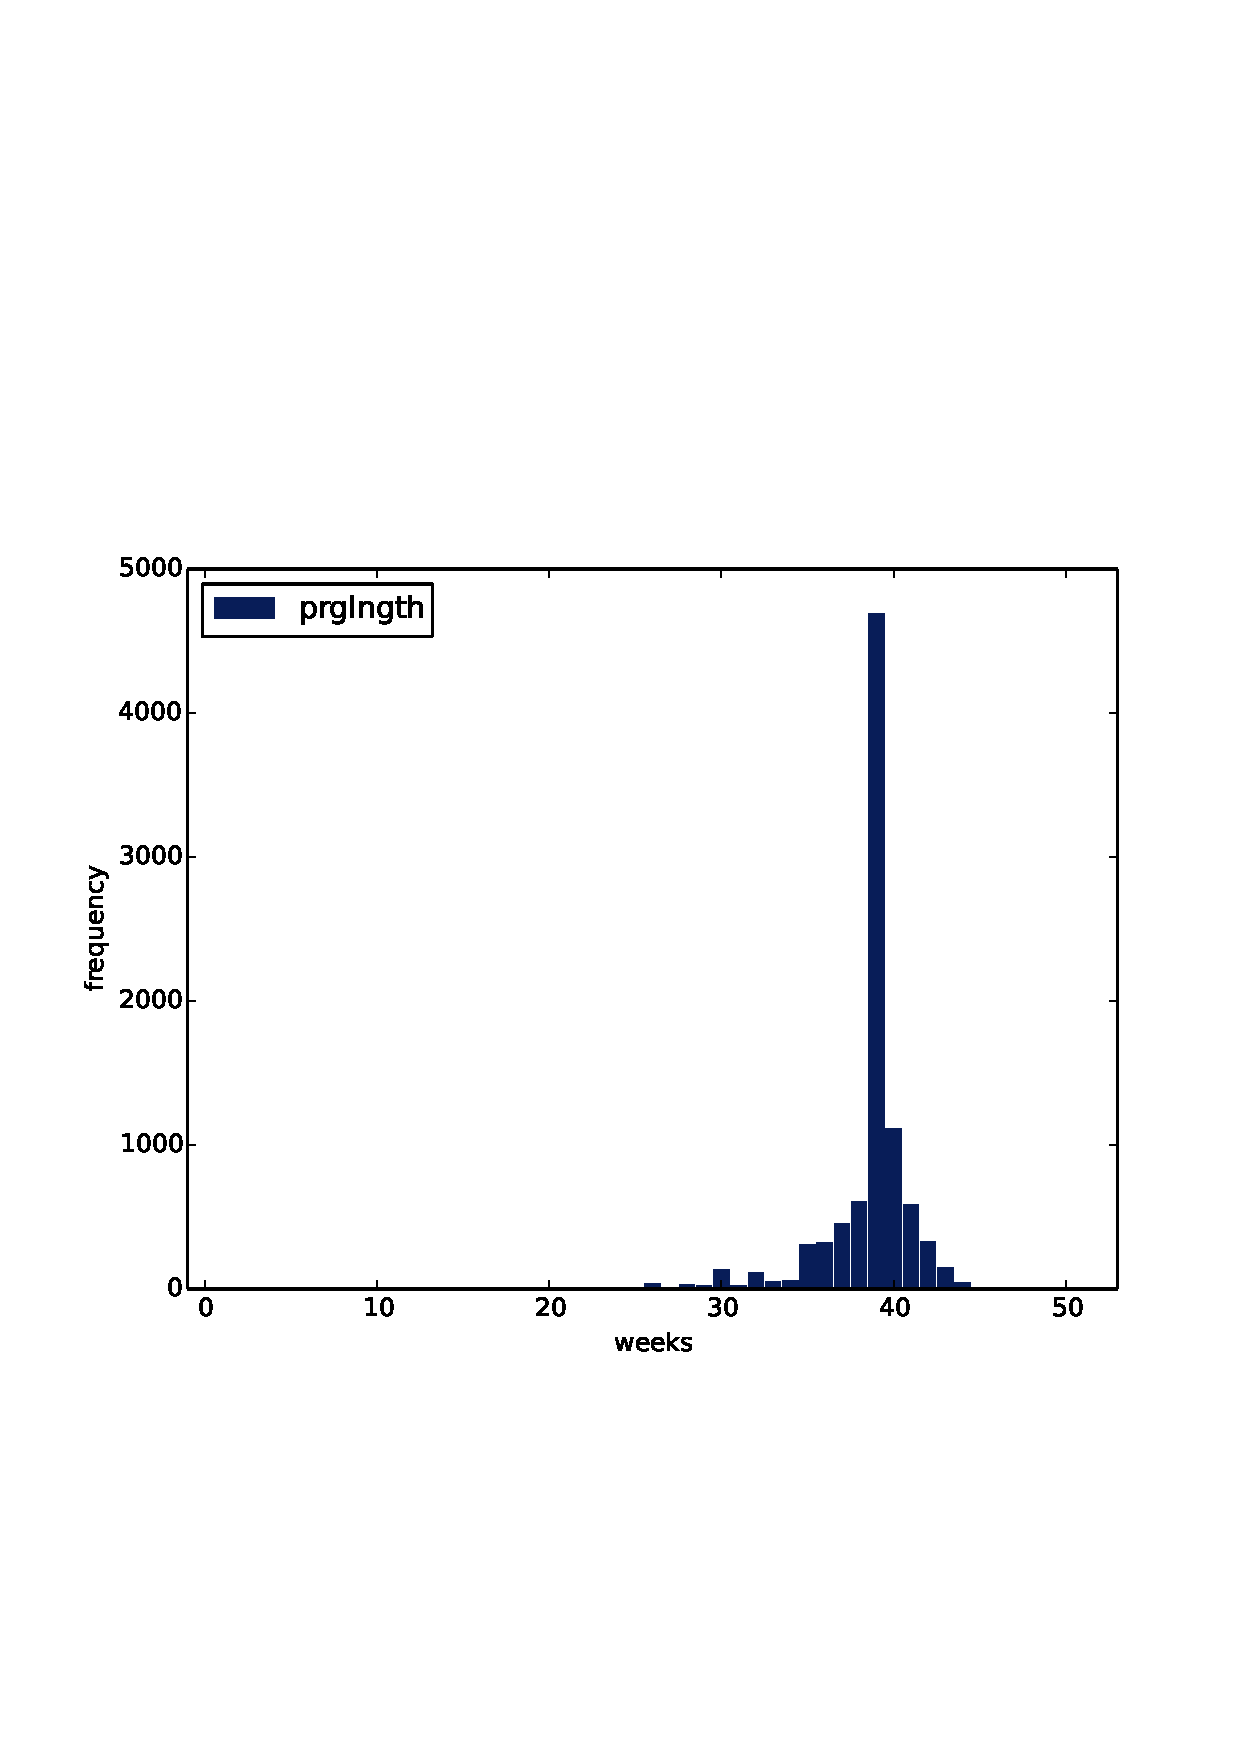
\includegraphics[height=2.5in]{figs/first_prglngth_hist.pdf}}
\caption{임신기간(주별) 히스토그램.}
\label{first_prglngth_hist}
\end{figure}

그림~\ref{first_wgt_lb_hist}가 결과를 보여준다.
가장 많이 관찰되는 값을 {\bf 최빈값(mode)}이라고 하고 이 경우에 7 파운드다. 
분포는 근사적으로 종모양인 {\bf 정규(normal)} 분포 모양으로 
{\bf 가우스(Gaussian)} 분포라고도 한다. 하지만, 순수 정규분포와 달리,
분포가 비대칭이다; 오른쪽보다 왼쪽으로 좀더 확장된 {\bf 꼬리(tail)}가 있다.


그림~\ref{first_wgt_oz_hist}은 변수 \verb"birthwgt_oz"의 히스토그램으로 출생 체중의 온스 부분이다. 
이론적으로 분포가 {\bf 균등(uniform)}하길 기대한다; 즉, 모든 값이 동일한 빈도를 가져야 한다.
사실 0 이 다른 값과 비교하여 좀더 흔하고, 1과 15는 좀더 흔하지 않은데, 아마도 이유는 응답자가 정수값에 가까운 출생 체중을 반올림한것으로 추측한다.

\index{출생 체중 (birth weight)}
\index{체중 (weight)!출생 (birth)}

그림~\ref{first_agepreg_hist}은 \verb"agepreg"의 히스토그램으로 임신 말기 산모 나이다.
분포는 대략 종모양이지만, 이 사례의 경우 꼬리가 좀더 왼쪽보다 오른쪽으로 뻗여나갔다. 
대부분의 산모는 20대이지만 30대도 적은 수지만 존재한다.

 
그림~\ref{first_prglngth_hist}은 \verb"prglngth"의 히스토그램으로 주간(week) 단위 임신기간이다.
가장 흔한 값은 39주다. 외쪽 꼬리가 오른쪽 꼬리보다 길다; 조산 신생아가 일반적이지만,
임신기간이 43주를 넘어가지는 않고, 만약 의사가 판단하기에 필요하다면 임신기간에 관여하는 것이 일반적이다.

\index{임신 기간 (pregnancy length)}


\section{특이점 (Outliers)}

히스토그램을 보면, 가장 흔한 값과 분포 모양을 식별하기는 쉽다. 하지만, 드문 값이 항상 눈에 잘 뜨이지는 않는다.
\index{히스토그램 (histogram)}

계속 진행하기 전에, {\bf 특이점 (outliers)}을 점검하는 것이 좋은 생각이다. 특이점은 이상치라고 불리는 극단값으로 측정과 기록에서 오류일 수도 있고, 드분 사건의 정확한 기록일 수도 있다.

\index{특이점 (outlier)}

Hist는 {\tt Largest}, {\tt Smallest} 메쏘드를 제공하는데, 정수 {\tt n}을 받아 히스토그램에서 최대값과 최소값 {\tt n}개를 반환한다.

\index{Hist}

\begin{verbatim}
    for weeks, freq in hist.Smallest(10):
        print(weeks, freq)
\end{verbatim}

정상 출산에 대한 임신기간 리스트에서 가장 작은 최소값 10개는 {\tt [0, 4, 9, 13, 17, 18, 19, 20, 21, 22]}이다. 10 주보다 적은 값은 확실한 오류다; 가장 그럴듯한 설명은 아마도 결과를 올바르게 코드화하지 못한 것이다. 30주 이상되는 값은 아마도 적합하다. 10주에서 30주 사이의 값은 확실하다고 하기가 어렵다; 몇몇 값은 아마도 오류지만 몇몇은 미숙아를 나타낸다.

\index{임신 기간 (pregnancy length)}

범위의 반대편에서 가장 큰 값은 다음과 같다.

%
\begin{verbatim}
weeks  count
43     148
44     46
45     10
46     1
47     1
48     7
50     2
\end{verbatim}

만약 임신기간이 42주를 넘어가면 대부분의 의사는 유도분만(induced labor)을 추천한다.
그래서 몇몇 긴 임신기간값은 놀라움을 준다. 특히, 임신 50주는 의학적으로 가능하지 않아 보인다.

특이점을 다루는 가장 좋은 방법은 ``특정 분야의 전문 지식(domain knowledge)''에 달려있다; 즉, 데이터 출처와 데이터가 의미하는 바에 대한 정보. 그리고 어떠한 분석방법을 수행할지에 달려있다.

\index{특이점 (outlier)}

이번 예제에서, 동기 부여 질문은 첫번째 아이가 일찍 (혹은 늦게) 태어나는 경향이 있느냐는 것이다.
사람들이 이 질문을 할 때, 대체로 전체 임신기간에 관심이 있다. 그래서, 이번 분석에서는 27주 이상이 되는 
임신에 초점을 맞출 것이다. 


\section{첫번째 아이 (First babies)}

첫째 아이와 나머지 아이에 대한 임신 기간 분포를 이제 비교할 수 있다.
{\tt birthord} 변수를 사용해서 정상 출산 데이터프레임을 나누고 히스토그램을 연산해서 그린다.

\index{데이터프레임 (DataFrame)}
\index{Hist}
\index{임신 기간 (pregnancy length)}

\begin{verbatim}
    firsts = live[live.birthord == 1]
    others = live[live.birthord != 1]

    first_hist = thinkstats2.Hist(firsts.prglngth)
    other_hist = thinkstats2.Hist(others.prglngth)
\end{verbatim}

그리고 나서, 동일 축에 히스토그램을 플롯하여 그린다.

\begin{verbatim}
    width = 0.45
    thinkplot.PrePlot(2)
    thinkplot.Hist(first_hist, align='right', width=width)
    thinkplot.Hist(other_hist, align='left', width=width)
    thinkplot.Show(xlabel='weeks', ylabel='frequency')
\end{verbatim}

{\tt thinkplot.PrePlot} 함수는 그래프를 그리려고하는 히스토그램 갯수를 인자로 받는다;
인자 정보를 이용해서 적절한 색깔 집합을 선택할 수 있다.

\index{thinkplot}

\begin{figure}
% first.py
\centerline{\includegraphics[height=2.5in]{figs/first_nsfg_hist.pdf}}
\caption{임신기간 히스토그램.}
\label{first_nsfg_hist}
\end{figure}

{\tt thinkplot.Hist}는 {\tt align='center'}을 기본값으로 사용해서 
각 막대는 값에 대해서 중앙에 위치한다. 그림에서는 {\tt align='right'}와 {\tt align='left'}를
사용해서 각 값의 양쪽으로 해당 막대를 위치시켰다.
\index{Hist}

{\tt width=0.45} 옵션값으로, 두 막대의 전체 넓이는 0.9로, 각 막대페어 간에 약간 공백을 두었다.

마지막으로, 축을 조정해서 27주와 46주 사이 데이터만 보이게 만들었다. 
그림~\ref{first_nsfg_hist}이 지금까지의 결과를 보여준다.
\index{임신 기간 (pregnancy length)}
\index{기간 (length)!임신 (pregnancy)}

히스토그램은 최빈값을 즉시 명확하게 보여준다는 점에서 유용하다.
하지만, 두 분포를 비교하는데는 가장 좋은 선택이 되지는 못하다. 
이번 예제에서 ``첫째가 아닌 아이''보다 ``첫째 아이'' 숫자가 더 적다. 
그래서, 히스토그램에서 명백한 차이는 표본크기에서 나온다. 다음 장에서 확률질량함수(probability mass functions)를 사용해서
이 문제를 다뤄본다. 


\section{분포 요약하기}
\label{mean}

히스토그램은 표본을 완전히 기술하는 분포다; 즉, 히스토그램이 주어진다면 (순서대로는 할 수 없지만) 표본에 있는 값을 재구성할 수 있다.

만약 분포에 대한 자세한 사항이 중요하다면, 히스토그램으로 표현하는 것이 필요할지도 모른다.
하지만, 종종 기술 통계량 몇개로 분포를 요약할 때도 있다.

보고하는데 사용되는 특성치 몇개는 다음과 같다.

\begin{itemize}

\item 중심경향성 (central tendency): 
값들이 특정한 점을 주심으로 군집하는 경향이 있는가?
\index{중심경향성 (central tendency)}

\item 모드 (modes): 하나 이상 군집(cluster)이 있는가?
\index{모드 (mode)}

\item 퍼짐 (spread): 값들에 얼마나 많은 변동이 있는가?
\index{퍼짐 (spread)}

\item 꼬리 (tails): 모드(최빈값)에서 멀어질 때, 확률이 얼마나 빨리 떨어지는가?
\index{꼬리 (tail)}

\item 특이점 (outliers): 모드(최빈값)에서 멀리 떨어진 극단값이 있는가?
\index{특이점 (outlier)}

\end{itemize}

상기 질문에 대답하도록 설계된 통계량이 {\bf 요약통계 (summary statistics)}다.
지금까지 가장 흔한 요약통계는  {\bf 평균(mean)}으로 분포의 중심경향성을 기술하는 의도가 있다.
\index{평균 (mean)} 
\index{평균 (average)} 
\index{요약통계 (summary statistic)}

각 값이 $x_i$인 {\tt n}개 표본이 있다면, 평균 $\xbar$는 값을 합한 뒤에 표본갯수로 나눈 것이다;
다른 말로, 
%
\[ \xbar = \frac{1}{n} \sum_i x_i \]
%

``평균 (mean)''와 ``평균(average)''은 때때로 상호호환적으으로 사용된다. 하지만 다음과 같이 이 책에서 구별한다.


\begin{itemize}

\item 표본 ``평균 (mean)''은 앞선 공식으로 계산되는 요약 통계다.

\item ``평균 (average)''은 중심경향성을 기술하려고 선택하는 다수 요약통계량 중 하나다.
\index{중심 경향성 (central tendency)}

\end{itemize}

때때로 평균(mean)은 값들의 집합을 잘 기술한다. 예를 들어, 사과는 거의 크기가 동일하다. (최소한 마트에서 팔리는 사과는 그렇다.)
그래서, 사과 6개를 사고, 전체 무게가 3 파운드라면, 사과 각각은 0.5 파운드라고 주장하는 것은 일리있는 요약이 된다. 

\index{무게 (weight)!호박 (pumpkin)}

하지만, 호박은 좀더 다양하다. 텃밭에서 호박 몇종을 기른다고 가정하자.
어느날 1 파운드 장식용 호박 3개, 3 파운드 호박파이용 호박 2개, 그리고 519 파운드 대서양 거인 호박 한개를 수확했다.
표본 평균은 100 파운드다. 하지만, ``텃밭에 호박 평균 무게는 100 파운드''라고 말한다면 오도할 수 있다.
호박 무게에 대해서 전형적인 호박이 없기 때문에 유의미한 평균은 없다.

\index{호박 (pumpkin)}


\section{분산 (Variance)}
\index{분산 (variance)}

호박 무게를 요약하는 단 하나의 숫자가 없다면, 숫자 두개로 좀더 잘 할 수 있다; 평균(meand)과 
{\bf 분산 (variance)}.

분산은 분포의 변동(variability)과 퍼짐(spread)을 기술하려는 요약통계다. 
값들의 집합에 대한 분산은 다음과 같다.

%
\[ S^2 = \frac{1}{n} \sum_i (x_i - \xbar)^2 \]
%

$x_i - \xbar$ 항은 ``평균으로부터 편차(deviation from the mean)''라고 하고,
분산은 평균제곱편차다. 분산의 제곱근($S$)을 {\bf 표준편차 (standard deviation)}라고 한다.
\index{편차 (deviation)}
\index{표준편자 (standard deviation)}

이전에 경험이 있다면, 분모에 {\tt n} 대신에 $n-1$로 분산을 계산하는 공식을 봤을 것이다.
이 통계치는 표본을 사용해서 모집단 분산을 추정하는데 사용된다. 이것에 대해서는 나중에 ~\ref{estimation}장에서 
다시 다룰 것이다.
\index{표본 분산 (sample variance)}

판다스 자료구조는 평균, 분산, 표준편차를 계산하는 메쏘드를 제공한다.
\index{판다스 (pandas)}

\begin{verbatim}
    mean = live.prglngth.mean()
    var = live.prglngth.var()
    std = live.prglngth.std()
\end{verbatim}

모든 정상 분만에 대해서, 평균 임신기간은 38.6주, 표준편차는 2.7주로 의미하는 바는 일반적으로 2-3주 편차가 있다는 것이다.
\index{임신 기간 (pregnancy length)}

임신 기간의 분산은 7.3으로 해석하기가 여렵다. 특히, 단위가 주$^2$, 즉 ``주 제곱''이다.
분산은 몇몇 계산에서는 유용하지만, 좋은 요약통계는 아니다.


\section{효과 크기 (Effect size)}
\index{효과 크기 (effect size)}

{\bf 효과 크기(effect size)}는 효과의 크기를 기술하려는 요약 통계다. 예를 들어,
두 집단간에 차이를 기술하기 위해서 평균값의 차이는 명확한 한가지 선택이 된다.
\index{효과 크기 (effect size)}

첫째 아이에 대한 평균 임신기간은 38.601; 첫째를 제외한 아이들의 평균 임신기간은 38.523이다. 
차이는 0.078주가 되고, 시간으로는 13시간이다. 전형적인 임신기간에 대한 일부분으로 보면, 차이는 약 0.2\%가 된다.
\index{임신 기간 (pregnancy length)}

만약 추정치가 정확하다고 가정하면, 이와 같은 차이는 실질적인 중요성은 없다.
사실, 대규모 임신사례를 관찰하지 않고 누구도 이와 같은 차이를 인지할 것 같지는 않다.
\index{효과 크기 (effect size)}

효과의 크기를 전달하는 또 다른 방법은 집단간(between groups)의 차이를 집단내(within groups) 변동성과 비교하는 것이다. 코헨(Cohen) $d$가 이러한 의도를 가진 통계량이다; 다음과 같이 정의된다.

%
\[ d = \frac{\bar{x_1} - \bar{x_2}}{s}  \]
%

$\bar{x_1}$와 $\bar{x_2}$은 집단 평균값이고, $s$는 ``합동 표준편차(pooled standard deviation)''다.
코헨(Cohen) $d$를 계산하는 파이썬 코드가 다음에 있다.

\index{표준편차 (standard deviation)!합동 (pooled)}

\begin{verbatim}
def CohenEffectSize(group1, group2):
    diff = group1.mean() - group2.mean()

    var1 = group1.var()
    var2 = group2.var()
    n1, n2 = len(group1), len(group2)

    pooled_var = (n1 * var1 + n2 * var2) / (n1 + n2)
    d = diff / math.sqrt(pooled_var)
    return d
\end{verbatim}

이 예제애서, 평균값의 차이는 0.029 표준편차로 크지 않다. 이러한 관점에서 본다면,
남성과 여성의 키 차이는 약 1.7 표준편차다.(\url{https://en.wikipedia.org/wiki/Effect_size} 참조)


\section{결과 보고하기}

첫째 아이와 첫째가 아닌 아이간에 임신 기간(만약 차이가 있다면)에 
차이를 기술하는 몇가지 방법을 살펴봤다.
\index{임신 기간 (pregnancy length)}

질문은 누가 질문을 하느냐에 달려있다. 과학자는 아무리 작더라도 존재하는 (실제) 차이에 관심이 있을지 모른다. 의사는 단지 {\bf 임상적으로 유의한 (clinically significant)} 효과에만 관심을 둘 수 있다; 즉, 치료결정에 영향을 주는 차이. 임신한 여성은 늦게 혹은 빨리 출산할 확률 같은 본인에게 관련된 결과에만 관심이 있을 수 있다. 

\index{임상적으로 유의한 (clinically significant)}
\index{유의한 (significant)}

어떻게 결과를 보고할지도 또한 목적에 달려있다. 만약 효과의 중요성을 시연하려고 한다면,
차이를 강조하는 요약통계량을 선택할 수도 있다. 만약 환자를 안심시키고자 한다면, 차이를 염두에 둔 통계량을 선택할지도 모른다. 

물론, 본인의 결정은 또한 전문가 윤리에 따라야만 한다. 설득하려고 한다면 괜찮다; 
스토리를 명확하게 전달하는 시각화 도구와 통계 보고서를 설계{\em 해야만 한다.}
하지만, 또한 보고서를 정직하게 만들고, 불활실성과 한계를 인정하는데도 최선을 다해야 한다.

\index{윤리 (ethics)}


\section{연습 문제}

\begin{exercise}
이번 장의 결과에 기반해서, 첫번째 아이 출산이 늦은가에 관해서 배운 것을 요약하도록 요청받는다고 가정하자.

9시 뉴스에 나온다면, 어떤 요약 통계량을 사용해야 할까?
불안해 하는 환자를 안심시키려면 어떤 요약 통계량을 사용해야 할까?

\index{Adams, Cecil}
\index{Straight Dope, The}

마지막으로, {\it 진실한 정보(The Straight Dope)} (\url{http://straightdope.com})의 저자
세실 아담스(Cecil Adams)라고 상상하자. 여러분의 일은 ``첫째 아이가 늦게 태어나는가?'' 질문에 대답하는 것이다.
분명하고, 정확하고, 정직하게 질문에 답하는데 이번 장에서 나온 결과를 사용해서 한 문단으로 작성하시오.
\index{윤리}

\end{exercise}

\begin{exercise}
다운로드받은 저장소에서, \verb"chap02ex.ipynb" 라는 이름의 파일을 찾아서 연다.
일부 셀이 이미 채워져 있고, 채워진 셀은 실행해야 한다.
다른 셀은 연습문제로 명령어를 넣어 주어야 된다.
지침을 따라서 정답을 채워넣으세요.

연습문제에 대한 해답은 \verb"chap02soln.ipynb" 파일에 나와 있다.

\end{exercise}

다음 연습문제로, {\tt chap02ex.py} 이름으로 파일을 생성하시오.
\verb"chap02soln.py" 파일에 정답이 나와있다.

\begin{exercise}
분포 최빈값(mode)은 가장 빈번하게 나오는 값이다; 
\url{http://wikipedia.org/wiki/Mode_(statistics)}을 참조한다.  
Hist를 입력값으로 받아서 가장 빈번하게 나오는 값을 반환하는 함수 
{\tt Mode}를 작성하시오.

\index{최빈값}
\index{Hist}

좀더 도전적인 연습문제로, {\tt AllModes}라는 함수를 작성한다.
빈도수를 내림차순으로 정렬하는 값-빈도를 짝지은 목록으로 반환한다.
\index{빈도}
\end{exercise}

\begin{exercise}
변수 \verb"totalwgt_lb"을 사용해서, 첫번째 아이가 다른 아이들보다 더 가벼운지
더 무거운지 조사하시오. 집단 사이 차이를 정량화하는데 코헨 $d$ (Cohen's $d$)를 계산한다.
임신 기간에 차이와 어떻게 비교가 되는가?
\index{임신 기간}
\end{exercise}


\section{용어사전}

\begin{itemize}

\item 분포 (distribution): 표본에 나타나는 값과 개별 값의 빈도
\index{분포 (distribution)}

\item 히스토그램 (histogram): 값에서 빈도로 매핑, 혹은 매핑을 보여주는 그래프.
\index{히스토그램 (histogram)}

\item 빈도 (frequency): 표본에서 값이 나타나는 횟수.
\index{빈도 (frequency)}

\item 최빈값 (mode): 표본에서 가장 빈도가 높은 값 혹은 가장 빈도가 높은 값중의 하나.
\index{최빈값 (mode)}

\item 정규분포 (normal distribution): 이상적인 종모양 분포; 가우스 분포로도 알려져 있다.
\index{가우스 분포 (Gaussian distribution)}
\index{정규분포 (normal distribution)}

\item 균등분포 (uniform distribution): 모든 값이 동일한 본도를 갖는 분포.
\index{균등분포 (uniform distribution)}

\item 꼬리 (tail): 가장 높고 가장 낮은 극단에 있는 분포 부분.
\index{꼬리 (tail)}

\item 중심경향성 (central tendency): 표본 혹은 모집단 특성치; 직관적으로 평균 혹은 전형적인 값.
\index{중심경향성 (central tendency)}

\item 특이점 (outlier): 중심경향성에서 떨어진 값.
\index{특이점 (outlier)}

\item 퍼짐 (spread): 분포에 있는 값들이 얼마나 퍼져있는지에 대한 측정.
\index{퍼짐 (spread)}

\item 요약통계 (summary statistic): 
중심경향성 혹은 퍼짐같이 분포의 일부 측면을 정량화하는 통계치.
\index{요약통계 (summary statistic)}

\item 분산 (variance): 퍼짐을 정량화하는데 종종 사용되는 요약통계.
\index{분산 (variance)}

\item 표준편차 (standard deviation): 분산의 제곱근으로 또한 퍼짐을 측정하는데 사용된다.
\index{표준편차 (standard deviation)}

\item 효과 크기 (effect size): 집단간의 차이처럼 효과 크기를 정량화하는 요약통계.
\index{효과 크기 (effect size)}

\item 임상적으로 유의한 (clinically significant): 집단간 차이처럼, 실제로 연관있는 결과. 
\index{임상적으로 유의한 (clinically significant)}

\end{itemize}



